% ::setlocal makeprg=cd\ presentazione\ &&\ pdflatex\ -interaction=batchmode\ main.tex\ &&\ xdg-open\ main.pdf\ &

\section{Capitolo 2}

\begin{frame}{Simulazione}

    Equazioni del moto per una particella massiva

	\begin{align*}[left = {\empheqlbrace}]
        &\frac{1}{2} \left(\dv{r}{\tau}\right)^2 = \mathcal E - V_{\rm eff} (r) \\
        &\dv{\phi}{\tau} = \frac{l}{r^2} \\
        &\dv{t}{\tau} = \frac{e}{1 - 2 M / r}
	\end{align*}

\end{frame}


\begin{frame}{Video on the computer}
    \centering
    \movie[externalviewer]{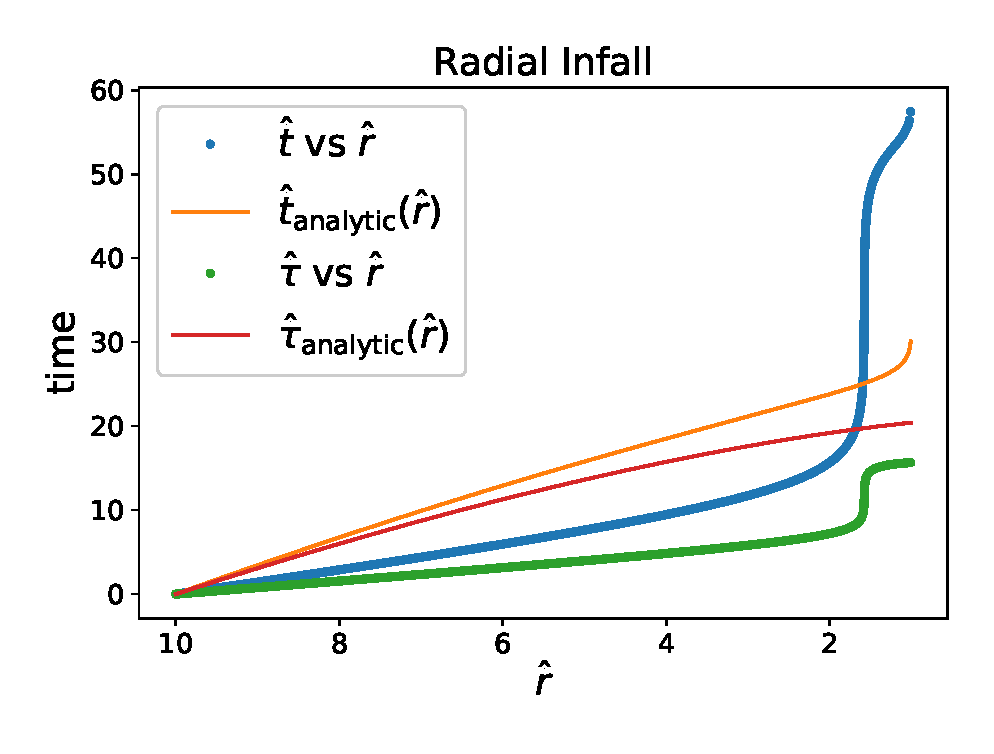
\includegraphics[width=\textheight, keepaspectratio]
    {Videos/infall.png}}{Videos/infall.mov}
\end{frame}


\begin{frame}{Video on the computer}
    \centering
    \movie[externalviewer]{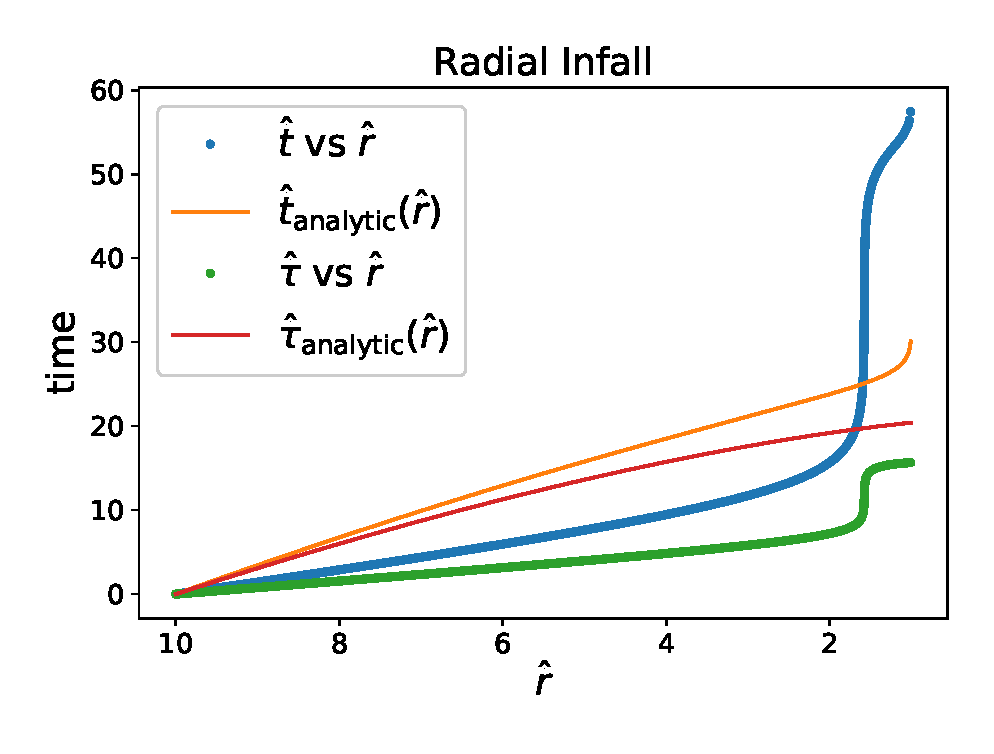
\includegraphics[width=\textheight, keepaspectratio]
    {Videos/infall.png}}{Videos/infall.mp4}
\end{frame}


\begin{frame}{Video on the computer}
    \centering
    \movie[externalviewer]{\includegraphics[width=\textheight, keepaspectratio]
    {Videos/volevi.png}}{Videos/volevi.mov}
\end{frame}


\begin{frame}{Video on the computer}
    \centering
    \movie[externalviewer]{\includegraphics[width=\textheight, keepaspectratio]
    {Videos/precession.png}}{Videos/precession.mp4}
\end{frame}


\begin{frame}{Video on the computer}
    \centering
    \movie[externalviewer]{\includegraphics[width=\textheight, keepaspectratio]
    {Videos/precession2.png}}{Videos/precession2.mp4}
\end{frame}


\begin{frame}{Video on the computer}
    \centering
    \movie[externalviewer]{\includegraphics[width=\textheight, keepaspectratio]
    {Videos/precession2.png}}{Videos/precession2.MOV}
\end{frame}


\begin{frame}{Video on the computer}
    \centering
    \movie[externalviewer]{\includegraphics[width=\textheight, keepaspectratio]
    {Videos/precession_ani.png}}{Videos/precession_ani.mov}
\end{frame}
